\chapter{Matériels et Méthodes}

Méthode CRISP\cite{crisp}

Évaluation de nos modèles \cite{plasticc_team_2019_2539456}

\section{Compréhension du problème}
Étant la première tâche que nous avons réalisée, la phase de compréhension du problème est la première phase de gestion de projet de datamining. Cette première étape consiste à bien comprendre les éléments métiers et problématique que le datamining vise à résoudre ou à améliorer.
Pour mieux cerner la problématique et comprendre les objectifs à atteindre, nous allons débuter par contextualiser le problème.
\subsection{Contexte du problème}
Le développement de la théorie de la relativité générale couplée à de nombreuses observations astrophysiques ont permis l'élaboration d'un modèle, décrivant l'histoire de l'Univers, son évolution, son expansion et sa composition énergétique.
Les observations des galaxies et plus récemment, celles des supernovae, ont montré que notre univers est en expansion et même en expansion accélérée, ce qui ne peut se concevoir simplement compte-tenu de la force gravitationnelle qui tend à agglomérer la matière.
Du fait de l'expansion de l'Univers, les objets lointains voient leurs spectres décalés vers le rouge. La mesure de ce décalage (couramment nommé redshift) est une mesure indirecte de la distance à laquelle se trouve l'objet observé mais également une mesure du paramètre d'expansion, ce qui permet d'étudier les caractéristiques de l'énergie noire. Grâce à de nombreuses sondes observationnelles il est possible d'étudier l'évolution de l'Univers au cours du temps.
Afin d'obtenir les observations nécessaires, de nombreux projets ont vu le jour. Parmi eux, le \textbf{Large Synoptic Survey Telescope (LSST)} qui est un télescope grand champ qui devrait permettre l'observation de milliards de galaxies.
\subsection{Présentation du projet LSST (Large Synoptic Survey Telescope)}
Le projet LSST  est un projet international dont les objectifs de LSST balayent quatre thèmes de science à savoir :
\begin{itemize}
    \item La recherche et la compréhension de la matière noire.
    \item La recherche et la compréhension de l'énergie noire.
    \item L'étude des objets transitoires.
    \item L'étude de la Voie Lactée et du système solaire.
\end{itemize}
Chacun de ces thèmes va imposer des contraintes sur l'instrument et sa capacité d'observation.
Elles seront utilisées pour optimiser l'ensemble des paramètres caractéristiques du télescope.
\subsubsection{Présentation du télescope LSST}
\textbf{Le télescope LSST} est un télescope optique de grande taille en cours de construction au nord du Chili et caractérisé par un champ d’observation très large. Il observeras dans le domaine de l'optique, la totalité de l'hémisphère sud pendant plus de dix ans.
Son optique compacte sera composée de trois miroirs et une caméra avec un diamètre de 64 cm, 189 CCDs et plus de 3 milliards de pixels, sera la plus importante jamais construite. Son champ de vue à la fois large et profond va permettre l'étude de nombreux sujets scientifiques, de l'exploration intensive du système solaire aux mesures de précision des paramètres cosmologiques. 
Les mesures atmosphériques réalisées depuis 10 ans sur le site (depuis le Cerro Tololo Inter-American Observatory CTIO) montrent que plus de 80\% des nuits sont propices à l'observation avec d'excellentes conditions atmosphériques.
En plus des excellentes conditions d'observation, LSST bénéficiera d'une infrastructure (conditions d'accès ...) facilitée par la présence de télescopes d'envergure déjà en fonctionnement sur ce site. 
\newline
\newline
\begin{figure}[!h]
    \centering
    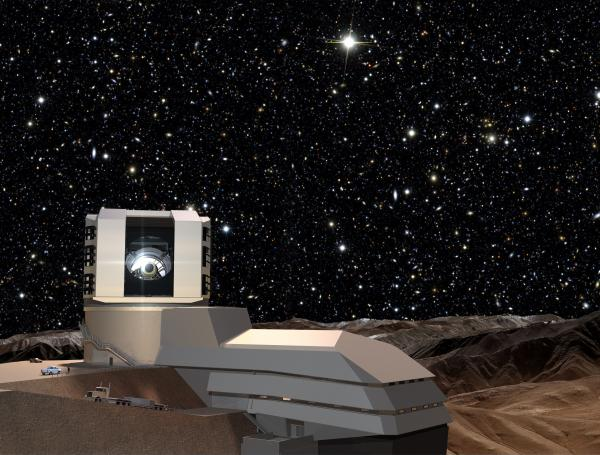
\includegraphics[width=12cm,height=7cm]{report/figures/LSST.jpg}
    \caption{Télescope LST}
    \label{fig:modeling_shema}
\end{figure}
\newline Il sera construit en tenant compte des paramètres définis sur le tableau ci-dessous.
\newline
\begin{tabular}{|p{10cm}|p{6cm}|}
\hline 
Paramètres & Valeurs \\
\hline 
 Site & Cerro Pachón Chili 1ère \\
\hline 
 1ère lumière & 2020 \\
\hline 
 Durée de vie nominale & 10 ans\\
\hline 
 Type de télescope & Paul Baker / Mersenne Schmidt grand champ \\
\hline 
Taille du sondage & 20 000 deg2 \\
\hline 
Champ de vue & 9.62 deg2 \\
\hline 
Longueur focale & 10.2 m Diamètre \\
\hline 
Diamètre effectif & 6.5 m \\
\hline 
Étendue & 319 m2/deg2 \\
\hline 
Résolution angulaire & 0.2 seconde d'arc / pixel\\
\hline 
Nombre de filtres & 6 (u g r i z y) \\
\hline 
Spectre photométrique & 310 à 1060 nm \\
\hline 
Durée d'exposition (tvis) & 30 s (2×15 s) \\
\hline 
Nombre de jours entre chaque visite & 3 à 4 \\
\hline 
Proportion du temps pour le programme principal & 90\% \\
\hline 
Proportion du temps pour les programmes spécifiques & 10\% \\
\hline
\end{tabular}
\subsubsection{La stratégie d'observation du télescope LSST}
Le principe fondamental de LSST est de balayer l'ensemble du ciel observable depuis le Chili avec un champ profond, large, et de manière rapide, avec une stratégie d'observation spécifique. Cette dernière est déterminée de façon à maximiser la qualité des observations scientifiques tout en minimisant les temps morts, avec une sélection appropriée du filtre en temps réel, et en fonction des conditions météorologiques. Bien que la stratégie d'observation ne soit pas encore complètement déterminée à ce jour, environ 90\% du temps devrait être consacré au sondage principal. Celui-ci, dit (Universal cadence), devrait conduire à la réalisation d’une base de données répondant à la plupart des objectifs de science.  Les 10\% restants seront consacrés à la réalisation de champs plus profonds, avec des temps entre deux visites très courts (∼ 1 minute), et à l'observation de régions particulières, tel que le plan de l'écliptique, le plan galactique ou les nuages de Magellan.
La cadence d'observation principale va générer un flux continu de données brutes avec une production d'environ 15 terabyte (TB) par nuit. On estime qu'après 10 ans de fonctionnement, 11 Data Release seront produites à partir d'un ensemble de données approchant 500 Pentabyte(PB) pour l'imagerie d'images et environs environ 50 PB pour les catalogues.
\subsubsection{Gestion de données collectées}
L'importance des volumes de données produites, l'aspect temporel des phénomènes observés et la complexité des processus traités imposent un traitement en temps réel et automatisé des données. Ainsi les données collectées par LSST seront automatiquement réduites en images et en catalogues par le système. Les données seront traitées en suivant trois niveaux :
\begin{itemize}
    \item Traitement en temps réel: archivage des images brutes générées pendant la nuit d'observation et émission des alertes (détections de nouvelles source, ou sources dont les propriétés ont changées depuis la dernière observation) dans les 60 secondes qui suivent la détection.
    \item Une fois par an, les données seront retraitées afin de fournir un catalogue et des images parfaitement calibrées (une calibration photométrique et astrométrique uniforme sur le catalogue sera fournie).
    \item Les produits de données de niveau 3 sont issu d'une combinaison des niveaux 1 et 2 afin de répondre à certaine problématiques scientifiques particulières. Le système de gestion des données (Data Management System DMS) va faciliter cette étape du traitement des données en créant des logiciels et des interfaces (API pour Application Programming Interfaces) permettant le développement des logiciels d'analyse.
\end{itemize}

L’une des principales difficultés que rencontreront les scientifiques est l’exploitation des données qui seront issues des observations.
Pour pallier à ces difficultés les concepteurs du projet LSST ont lancés le projet PLAsTiCC  Photometric LSST Astronomical Time-Series Classification Challenge) dont le but est de concevoir un modèle permettant de classer les objets observés par le télescope LSST.

\subsection{PLAsTiCC  (Photometric LSST Astronomical Time-Series Classification Challenge)}
Afin de faciliter l’exploitation de données collectées, LSST demande à Kaggle de l’aider à se préparer à la classification des données des nouvelles observations à travers une compétition. 
Le but de cette compétition est d’amener les concurrents  à construire un modèle de  classification qui permettra de classer  les sources  des objets astronomiques observés. 
Le modèle à construire doit tenir compte du fait que les données qui seront issues des observations astronomique ont une luminosité qui varie au cours du temps et forment une série temporelle.
Les organisateurs du challenge ont mis à la disposition des compétiteurs un jeux de données à partir duquel ils doivent construire le modèle.
Le jeux de données mis à notre disposition fera l’objet d’une étude détaillé dans la section qui suit.


\section{Compréhension des données}
La compréhension des données est l’une des étapes les plus importantes pour la réalisation d’un projet data mining elle vise à déterminer précisément les données à analyser, à identifier la qualité des données disponibles et à faire le lien entre les données
et leur signification d’un point de vue métier. La Data Science étant basée sur les données seules, les problèmes métiers relatifs à des données existantes, qu’elles soient internes ou externes, peuvent ainsi être résolus par la Data Science. Les données sont mises à
disposition sur kaggle-plasticc-challenge.

\subsection{présentation des données}
Pour la réalisation du projet l’équipe plasticc-challenge à mit à notre disposition deux table de données qui sont partagées en données de Test et données d’entraînements .
\newline
\newline
\textbf{[training/test]-set-metadata :} Informations sur les objets qui ne changent pas dans le temps, comme les coordonnées de l’objet, voici les attributs de cette table.
\begin{itemize}
    \item \textbf{object-id :} identifiant d’objet unique de type Integer.
    \item \textbf{ra :} désigne l’ascension droite d’un objet, qui est une coordonnée ciel : co-longitude en degrés de type Float qui est calculé à partir de la différence de la latitude et 90°.
    \item \textbf{ decl:} la déclinaison d’un objet dans le ciel ou co-latitude en degrés de type Float.
    \item \textbf{ gal-l :} désigne la longitude galactique en degrés de type Float.
    \item \textbf{gal-b : }désigne la latitude galactique d’un objet en degrés de type Float.
    \item \textbf{ ddf :} Un drapeau pour identifier l’objet comme provenant de la zone de levé DDF (avec la valeur DDF = 1 pour le DDF, DDF = 0pour le levé WFD). si les champs DDF sont contenus dans la totalité de la zone d’enquête de la DCE, les incertitudes des flux DDF sont bien moindres de type Booléen.
    \item \textbf{ hostgal-specz : }le redshift spectroscopique de la source (décalage vers le rouge). Il s’agit d’une mesure extrêmement précise du décalage vers le rouge, disponible pour l’ensemble d’entraînement et une petite fraction de l’ensemble d’essai de type Float, les objet qui sont de redshift=ൡ sont galactiques.
    \item \textbf{hostgal-photoz :} Redshift photométrique de la galaxie hôte de la source astronomique. Bien que cela soit censé être un proxy pour hostgal-specz, il peut exister de grandes différences entre les deux et doit être considéré comme une version beaucoup moins précise de hostgal-specz cet attribut est de type Float.
    \item \textbf{hostgal-photoz-err :} L’incertitude sur hostgal-photoz d’après les projections de l’enquête LSST cet attribut est de type Float.
    \item \textbf{distmod :} La distance à la source calculée à partir de hostgal-photoz et en utilisant la relativité générale qui est une théorie relativiste de la gravitation, c’est-à-dire qu’elle décrit l’influence sur le mouvement des astres de la présence de matière et, plus généralement d’énergie, en tenant compte des principes de la relativité restreinte, cet attribut est de type Float.
    \item\textbf{mwebv :} MW E (BV). cette «extinction» de la lumière est une propriété de la poussière de la voie lactée (MW) le long de la ligne de mire de la source astronomique et est donc fonction des coordonnées du ciel de la source ra, décl. Ceci est utilisé pour déterminer une gradation et un redimensionnement de la lumière provenant de sources astronomiques dépendant de la bande passante, de type FLOAT.
    \item\textbf{target :} c’est La classe de la source astronomique. Ceci est fourni dans les données de formation. le but du défi est de déterminer correctement la cible (attribuer correctement les probabilités de classification aux objets). Il existe une classe dans l’ensemble de test qui ne se produit pas dans l’ensemble d’apprentissage : class-99 sert de classe ”autre” pour les objets n’appartenant à aucune des 14 classes de l’ensemble d’apprentissage. Int8
    \end{itemize}


\newline
\textbf{[training/test]-set :} Série chronologique d’observations des objets. Mappe aux métadonnées via object-id.
\begin{itemize}
    \item \textbf{object-id :} Clé étrangère avec les métadonnées de type Int32
    \item \textbf{ mjd :} l’heure en date julienne modifiée (MJD) de l’observation. Peut être lu comme des jours depuis le 17 novembre 1858 Peut être converti au temps de l’époque Unix avec la formule unix-time = (MJD−40587)x 86400. Float64
    \item \textbf{passband :} Le nombre entier spécifique à la bande passante LSST, tel que u, g, r, i, z, Y = 0,1,2,3,4,5, dans lequel il a été visualisé. Int8
    \item \textbf{flux :} le flux mesuré (luminosité) dans la bande passante d’observation, indiqué dans la colonne de la bande passante. Ces valeurs ont déjà été corrigées pour tenir compte de l’extinction des poussières (mwebv), bien que les objets fortement éteints aient de plus grandes incertitudes ( flux-err) malgré la correction. Float32
    \item \textbf{flux-err :} l’incertitude sur la mesure du flux listée ci-dessus. Float32
    \item \textbf{ detected :} Si 1, la luminosité de l’objet est significativement différente au niveau 3-sigma par rapport au modèle de référence. Seuls les objets avec au moins 2 détections sont inclus dans le jeu de données de type Booléen
\end{itemize}
\newline
\subsection{Les attributs de la base de données les plus prometteurs}
L’une des questions les plus importantes est quels sont les attributs les plus pertinants qui nous permettent de faire une meilleure classification. tout d’abord nous nous intéressons à l’attribut qu’on doit prédire qui est \textbf{la classe target}, il y’a 14 classes différentes et la 15ème classe “la classe 99” sert de classe ”autre” pour les objets n’appartenant à aucune des 14 classes de l’ensemble d’apprentissage.
\newline
Autres attributs très importants sont les attributs qui permettent de positionner un objet dans le ciel comme :
\begin{itemize}
    \item Les coordonnées de l’objet \textbf{: ra ,decl, gal-l, gal-b}.
    \item Les attributs qui nous permettent de dire si un objet est galactique ou extragalactique :\textbf{ hostgal-photoz, hostgal-photoz}, un objet est galactique si le redshift=0 extragalactique sinon.

    \item L’attribut \textbf{distmod} qui nous donne la distance entre l’objet céleste et le point d’observation.
\end{itemize}

\begin{figure}[!h]
    \centering
    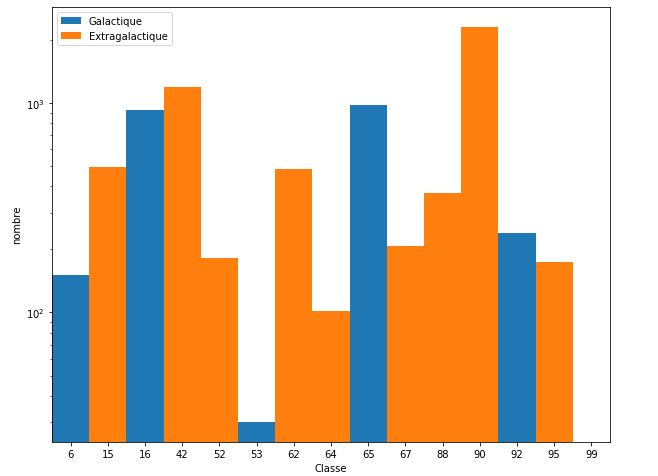
\includegraphics[width=12cm,height=7cm]{report/figures/galactic.jpg}
    \caption{table des corrélation entre attributs}
    \label{fig:my_label}
\end{figure}

\newline
D’autres attributs nous permettent de mesurer la luminosité de chaque objet lors des observation selon plusieurs filtres :
\begin{itemize}
    \item \textbf{passband, flux, flux-erreur}.
\end{itemize}
\newline
L’observation est faites sur des séries temporelles, la luminosité et la position d’un objets varie selon le temps, l’attribut utilisé ici est le \textbf{mjd}, qui est l’heure en date julienne modifiée.

\subsection{Les attributs qui semblent sans intérêt et peuvent être exclus}
certain attributs peuvent êtres exclus pour la modélisations car ils peuvent nous fausser les résultats, comme les attributs identifiant, ou les attributs aui nous permettent pas de faire une bonne classification, dans notre cas la plupart des attributs sont important, mais on peut mettre en vue certain autres comme :
\begin{itemize}
    \item \textbf{id-object }: qui est l’identifiant d’un objet dans une classe et qui sert de clés entre les deux table data et meta-data.
    \item \textbf{detected }: de type booléen, Seuls les objets avec au moins ൣ détections sont inclus
dans le jeu de données.
\end{itemize}
\subsection{corrélations entres attributs}
\newline
\begin{figure}[!h]
    \centering
    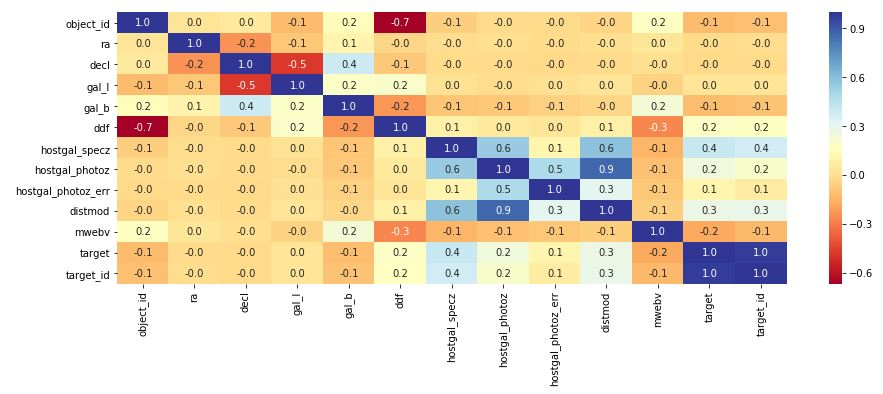
\includegraphics[width=12cm,height=7cm]{report/figures/correlation.jpg}
    \caption{table des corrélation pour les meta_data}
    \label{fig:my_label}
\end{figure}


\begin{figure}[!h]
    \centering
    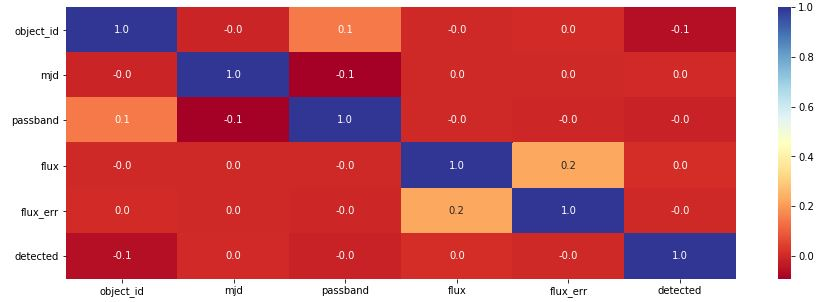
\includegraphics[width=12cm,height=7cm]{report/figures/correlation1.jpg}
    \caption{table des corrélation pour les data-est}
    \label{fig:my_label}
\end{figure}


\newpage
\subsection{}




















\section{Préparation des données}
Dans la section de préparation des données, on parlera des étapes qu’on avait réalisé pour obtenir nos données de la modélisation.
\subsection{Sélection des données}
\textbf{Choix des colonnes} : Dans les Meta data, on a les deux colonnes \textbf{hostgal-specz} et\textbf{ hostgal-photoz} présentant la même donnée mes en utilisant deux manière mesure différentes. Les données de la colonne \textbf{hostgal-specz} ne sont pas disponibles pour les données de test donc il faut l’éliminer. On aussi la colonne \textbf{MWEBV} qui n’est pas significative pour notre modèle. Pour les données, on a considéré comme hypothèse que toutes les colonnes seront utiles pour notre modélisation.
\subsection{Génération des données manquantes}
 Dans notre data set on un nombre important des données manquantes. On a supposé que le fait d’avoir des données manquantes impactera négativement notre tache de prédiction. Donc on va prédire ces valeurs avant de passer à la phase de construction de nouveau features pour notre modélisation. Pour faire cela on a utilisé les processus gaussiens. Dans cette méthode au lieu de créer une seule fonction  (dans le cas de régression), elle produit une distribution de toutes les fonctions possibles en fonction des points d'apprentissage. Pour ce faire, elle s’appuie sur la définition d’un processus gaussien, tel que « toute collection de variables aléatoires dans laquelle un sous-ensemble arbitraire de variables à une distribution gaussienne conjointe ». Cela signifie toutefois que la technique suppose que toutes les caractéristiques, y compris toutes les dimensions de x et y, ont une distribution gaussienne. Bien que cela semble limitant, cette hypothèse permet au système de s'exercer à l'aide de la matrice de covariance de la distribution jointe.
La figure \ref{fig:blackbox_shema} est une présentation du processus qu'on a développé pour la génération des données manquantes  des colonnes \textbf{flux} et \textbf{flux-error}.
\begin{figure}[!h]
    \centering
    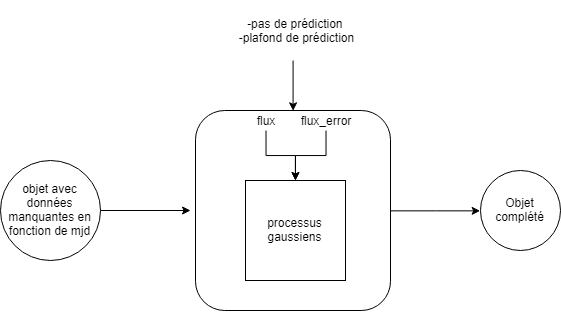
\includegraphics[width=12cm,height=7cm]{report/figures/blackbox.png}
    \caption{Schéma de prédiction des valeur manquante de flux et flux-error}
    \label{fig:blackbox_shema}
\end{figure}
\subsection{Génération de nouveaux features}



\section{Modélisation}

Les étapes précédentes nous ont permis de construire, à partir des données initiales, un data-set qui n'a plus de données manquantes et qui peut être utilisé pour entraîner des modèles de prédictions. Nous avons basé notre modélisation sur deux principales classes de modèles:
\begin{itemize}
    \item \textbf{Les modèles basés sur les caractéristiques :} Il s'agit ici de modèles qui se basent sur les méta données et sur les caractéristiques telles que la moyenne, les quartiles, la valeur maximale, la valeur minimale et bien d'autres pour faire les prédictions. Ces modèles supposent que les séries d'une même classes ont des caractéristiques similaires tandis que les séries de classes différentes ont des caractéristiques qui ne sont pas similaires.
    \item \textbf{Les modèles basés sur les similarités à des sous séries:} Ces modèles se basent sur l'hypothèse qu'il y a dans les séries temporelles des sous séquences qui sont représentatives pour la classes; ces sous-séquences sont appelées \textbf{shapelets} \citep{ye2009time}.
\end{itemize}
La figure \ref{fig:modeling_shema} est une représentation schématique du processus de modélisation que nous avons implémenté. Ce schéma va de l'acquisition des données jusqu'au modèle de prédiction. L'étape \textit{preprocessing} correspond à l'étape de préparation des données (Section \ref{sec:data_preparation}) dont le but était le traitement des valeurs manquantes et la normalisation des données. Les éléments suivant seront expliqués dans les lignes qui suivent selon qu'on soit orienté caractéristiques (Section \ref{sec:feature_based_model}) ou shapelet (Section \ref{sec:shapelet_based_model})

\begin{figure}[!h]
    \centering
    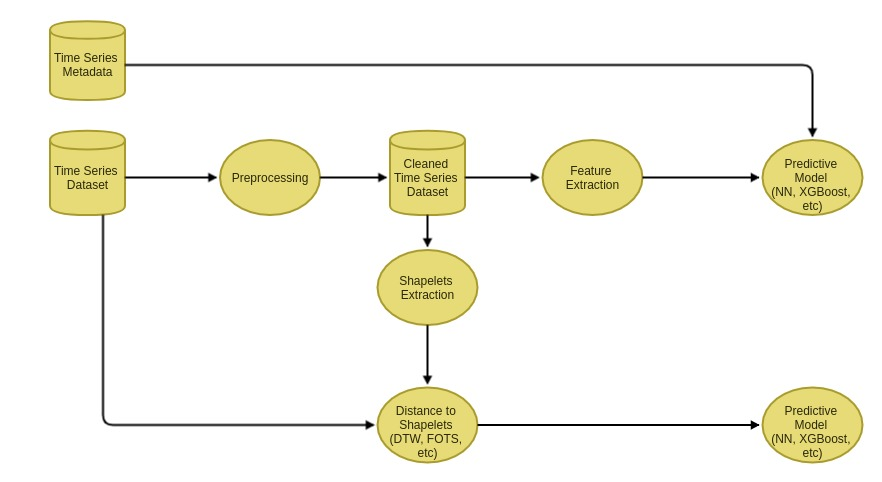
\includegraphics[width=12cm,height=7cm]{report/figures/modeling-schema.jpg}
    \caption{Schéma générale de modélisation}
    \label{fig:modeling_shema}
\end{figure}

\subsection{Modèles basés sur les caractéristiques}\label{sec:feature_based_model}

\subsection{Modèles basés sur les shapelets}\label{sec:shapelet_based_model}
Un Shapelet est défini comme une sous-séquence d'une série temporelle qui est représentative pour la classe \citep{ye2009time}. Ainsi une série temporelle appartient à une classe donnée si elle contient le \textit{shapelet} représentatif de ladite classe. Dans la pratique les séries d'une même classe n'ont pas exactement les mêmes sous-séquences représentatives mais elles ont des sous-séquences qui sont similaires aux sous-séquences représentatives de la classe. 
La classification des séries temporelles peut être réalisée par un arbre de décision (Figure \ref{fig:shapelet_based_dt}) dans lequel l'attribut de division (split) à chaque noeud est un \textit{shapelet} et les données sont séparées en fonction de leur similarité à ce \textit{shapelet}.

\begin{figure}[!h]
    \centering
    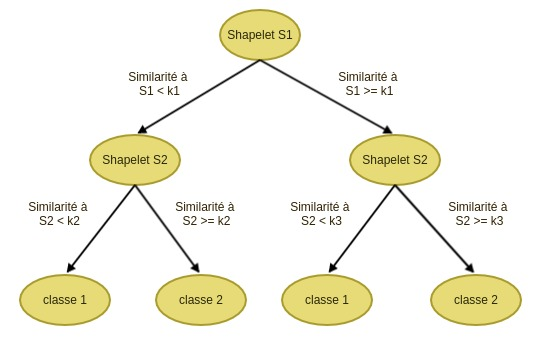
\includegraphics[width=10cm,height=7cm]{report/figures/shapelet-based-tree.jpg}
    \caption{Classification des séries temporelles basée sur les shapelets}
    \label{fig:shapelet_based_dt}
\end{figure}

La classification basées sur les shapelets a trois avantages \citep{ye2009time}:
\begin{itemize}
    \item les résultats sont interprétables 
    \item la robustesse: les shapelets sont des caractéristiques locales des séries temporelles. S'ils sont bien extraits, ils réduisent considérablement le bruit dans les données et rendent ainsi le modèle plus robuste
    \item la rapidité de classification: les shapelets étant des sous-séquences de taille généralement beaucoup plus petite que la taille des séries à classer, il est beaucoup plus rapide de comparer les séries aux shapelets que de comparer les séries entre elles.
\end{itemize}

Pour pourvoir appliquer ce modèle il faut pourvoir extraire les shapelets et définir la notion de similarité entre un shapelet et une série temporelle.

Commençons par donner quelques définitions formelles:

\textbf{Une série temporelle \textit{T}} est une ensemble ordonné de \textit{m} valeurs réelles. $ T = t_1, t_2,...,t_m $. \textit{m} est la taille de la séries.

\textbf{Une sous-série \textit{S} de \textit{T}} est un sous ensemble ordonné de \textit{l} ($ l \leq m $) valeurs de \textit{T}. $ S = T_p, T_{p+1},..., T_{p+l-1}, pour 1 \leq p \leq m-l+1 $. Le nombre de sous-séries peut très rapidement exploser lorsque $l$ est négligeable devant $m$. En effet une série de taille $m$ a exactement $ m-l+1 $ sous-séries de taille $l$. Les données de test de PLASTICC forment un ensemble de $ 3492890 $ de taille $1094$ chacune après qu'on l'imputation des valeurs manquantes. Le nombre de sous-séries possible est donc de $ 3492890 \times (1094 - l + 1)$, un algorithme naif serait donc inutilisable en pratique.

    \textbf{Un Shapelet} est une sous-séries qui permet de séparer l'ensemble des séries temporelles en deux classes suffisamment hétérogènes pour que l'une des classes contienne des séries qui ont une sous-séquence similaire au shapelet tandis que l'autre classe contient des séries qui n'ont pas de sous-séquence similaire au shapelet\cite{fotso2018frobenius}. 

\subsubsection{Mesure de la similarité}
Il existe dans la littérature plusieurs métriques pour mesurer la similarité entre deux séries temporelles de même taille. Nous avons par exemple la distance euclidienne, DTW (Dynamic Time Warping), DUST, PROUD, MUNICH et FOTS \cite{fotso2018frobenius}. Les séries temporelles de PLASTICC étant incertaines, FOTS serait la métrique la plus adaptée car elle est plus robuste à l'incertitude. Cependant, étant contraint par le temps, nous avons utilisé DTW car tslean l'implémente déjà et le calcul des valeurs propres dont a besoin FOTS sur un dataset aussi grand que celui de PLASTICC prendrait beaucoup trop de temps.

La similarité entre une séries $ T $ et une sous-séries $ S $ de taille inférieure ou égales est définie comme la similarité entre $ S $ et la sous-séries de $ T $ de même taille de de $ S $ et la plus similaire à $ S $. 
$$
Sim(S, T) = min \left \{ Sim(S, S'), |S|=|S'| \:  \forall S'\: sous \: séries \: de \: T \right \}
$$

Dans la formule précédente $ Sim $ peut être n'importe qu'elle mesure de similarité entre deux séries temporelles. 

\subsubsection{Extraction des shapelets}
Pour apprende les shapelets nous avons utilisé la bibliothèque tslean\citep{tslearn} qui implémente l'approche proposée par \citet{grabocka2014learning}. Cette approche considère la recherche des shapelets optimaux comme un problème d'optimisation qui débute par un choix aléatoire des shapelets puis les optimise au fur et à mesure en diminuant le taux d'erreur de classification. Le but est de ne pas rechercher dans l'ensemble des candidats possibles car trop grand. tslearn fournit également une heuristique qui permet de déterminer le nombre et la longueur de chacun des shapelets à apprendre. Selon cette heuristique, il nous a fallut apprendre sur les données de plasticc $ 109 $ shapelets de tailles $ 8 $ et $ 218 $ shapelets de tailles $ 7 $. La figure \ref{fig:shapelet_example} donne quelques shapelets que nous avons appris sur plasticc. Les couleurs correspondent aux différents filtres.

\begin{figure}[!h]
    \centering
    \begin{tabular}{c|c}
         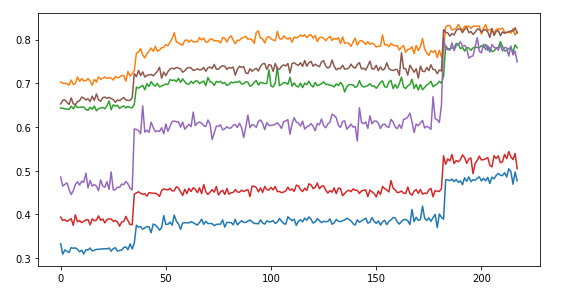
\includegraphics[width=7cm,height=5cm]{report/figures/shapelet.png} & 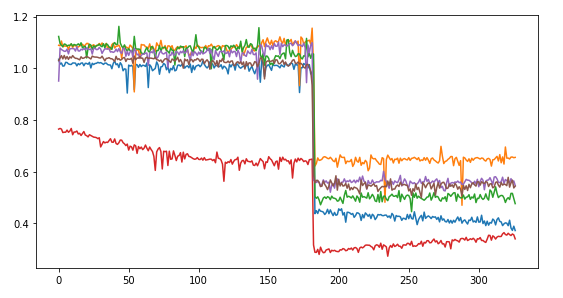
\includegraphics[width=7cm,height=5cm]{report/figures/shapelet2.png}
    \end{tabular}
    \caption{Exemple de shapelets appris sur PLASTICC}
    \label{fig:shapelet_example}
\end{figure}

\section{Évaluation}

\section{Déploiement}